\clearpage

\section{판정}\label{sec:oracle}

\subsection{문제 정의}

퍼징에서 가장 어려운 부분은 입력을 만드는 것이 아니라, \textbf{대상의 반응이 옳은지 판단하는 것}이다(판정 기준을 흔히 ``오라클''이라 부른다).
무작위로 변형한 입력도 여전히 유효한 요청일 수 있으므로, 응답만 보고는 결함 여부를 알 수 없다.

\begin{itemize}
    \item 다른 인증 태그로 인증 요청을 보냈더니 수락되었다 $\rightarrow$ 대상에 그 태그가 등록되어 있을 수 있으므로, 그 자체로는 결함이 아니다.
    \item 음수 커넥터 번호로 충전 시작을 요청했더니 수락되고 트랜잭션 번호가 발급되었다 $\rightarrow$ 잘못된 입력이 대상의 내부 상태를 실제로 바꾸었으므로 잠재 이슈이다.
    \item 형식이 깨진 메시지에 프로토콜 오류를 돌려주었다 $\rightarrow$ 올바른 방어 동작이다.
\end{itemize}

본 퍼저는 이 차이를 구분하기 위해 세 가지 정보를 함께 본다.

\begin{center}
\fbox{\begin{minipage}{0.9\textwidth}\centering\vspace{2pt}
(입력의 의도: 메시지 클래스) $\times$ (대상의 응답: 수락 / 거부 / 무응답) $\times$ (보호 상태의 변화)
\vspace{2pt}\end{minipage}}
\end{center}

\textbf{보호 상태}란 잘못된 입력으로 바뀌어서는 안 되는 대상의 핵심 상태로, 인증 여부, 트랜잭션 진행 여부와 번호, 커넥터, 세션 식별자를 말한다.

\subsection{판정 등급}

판정은 ``문제 없음''과 ``결함''의 이분법이 아니라, 증거의 강도에 따라 일곱 등급으로 나뉜다.
이를 통해 확실한 결함과 검토가 필요한 의심 동작, 그리고 시험 환경의 문제를 구분한다.

\begin{table}[H]
\centering
\small
\caption{판정 등급}
\label{tab:verdicts}
\begin{tabularx}{\textwidth}{l Y}
\toprule
\textbf{판정} & \textbf{의미} \\
\midrule
통과 & 문제가 발견되지 않음 \\
안전하게 거부됨 & 잘못된 입력을 프로토콜 오류로 안전하게 거부함 (바람직한 동작) \\
검토 필요 & 의심스럽지만 결론을 내리기 어려움 (무응답, 정책을 알 수 없는 수락 등) \\
잠재 이슈 & 잘못된 입력이 보호 상태를 바꾸는 등, 대상 측 결함 가능성이 높음 \\
실패 & 규격 위반이 확정됨 (형식이 깨진 응답, 정상 메시지의 거부 등) \\
설정 오류 & 연결 실패 등 퍼저나 시험 환경 쪽 문제 \\
잘못된 테스트 & 시험 구성 자체가 잘못되어 판정할 수 없음 \\
\bottomrule
\end{tabularx}
\end{table}

모든 판정에는 이유와 신뢰도(낮음/중간/높음), 그리고 판단에 사용한 근거(어떤 메시지에 어떤 응답이 왔고 상태가 어떻게 바뀌었는지)가 함께 기록된다.

\subsection{판정 절차}

판정은 그림~\ref{fig:oracle}의 순서로 이루어지며, 결론을 내린 첫 단계의 결과를 사용한다.

\begin{figure}[H]
\centering
\begin{tikzpicture}[node distance=4mm, every node/.style={font=\footnotesize}]
  \node[ext, minimum width=28mm] (in) {송수신 기록\\상태 흐름\\변형 의도 · 대상 정책};
  \node[box, right=8mm of in, minimum width=40mm] (e1) {\ding{172} 응답 형식 검사\\\scriptsize 규격에 맞는 응답인가, 요청과 짝이 맞는가};
  \node[box, below=of e1, minimum width=40mm] (e2) {\ding{173} 상태 불변식 검사\\\scriptsize 보호 상태가 부당하게 바뀌었는가};
  \node[box, below=of e2, minimum width=40mm] (e3) {\ding{174} 기대 반응과 비교\\\scriptsize 의도 대비 실제 반응};
  \node[box, below=of e3, minimum width=40mm] (e4) {\ding{175} 보조 신호\\\scriptsize 충전 중 연결 끊김 등};
  \node[ext, right=10mm of e2, minimum width=24mm, draw=ksred] (v) {판정\\\scriptsize 등급 · 이유\\\scriptsize 신뢰도 · 근거};
  \node[ext, below=of e4, minimum width=40mm] (p) {통과};
  \draw[arr] (in) -- (e1);
  \draw[arr] (e1) -- (e2); \draw[arr] (e2) -- (e3); \draw[arr] (e3) -- (e4); \draw[arr] (e4) -- node[lbl, right]{이상 없음} (p);
  \foreach \n in {e1,e2,e3,e4} { \draw[arr, ksred] (\n.east) -- (v.west); }
\end{tikzpicture}
\caption{판정 절차}
\label{fig:oracle}
\end{figure}

\begin{enumerate}
    \item \textbf{응답 형식 검사}: 응답이 규격에 맞는 형식인지, 보낸 요청과 짝이 맞는지, 핵심 메시지의 경우 응답 내용(필수 항목, 허용 값)까지 올바른지 확인한다.
    \item \textbf{상태 불변식 검사}: 요청 전후의 상태를 비교하여, 충전 세션이 지켜야 할 규칙이 깨졌는지 확인한다(\ref{subsec:invariants}절).
    \item \textbf{기대 반응과 비교}: 입력의 의도(메시지 클래스)로부터 기대되는 반응을 예측하고, 실제 응답 및 상태 변화와 비교한다(표~\ref{tab:matrix}).
    \item \textbf{보조 신호}: 충전 중 연결이 끊어지는 등, 위에서 걸러지지 않은 이상 징후를 검토 필요로 표시한다.
\end{enumerate}

웹 화면의 결과 상세 화면은 이 판정 과정을 \textbf{이 판정을 내린 방법}으로 그대로 보여 준다(그림~\ref{fig:ui-detail}).
그림의 예에서는 원격 충전 시작 명령의 커넥터 번호를 $-1$로 바꾸었고(형식은 맞지만 부적합한 메시지), 충전기가 이를 수락했지만 보호 상태 변화는 관찰되지 않았다.
따라서 결함으로 확정하지 않고 \textbf{검토 필요}로 판정했다. 화면 아래쪽에는 주고받은 메시지 원문이 시간순으로 표시되어, 검토자가 실제 교환 내용을 직접 확인할 수 있다.

\begin{figure}[H]
    \centering
    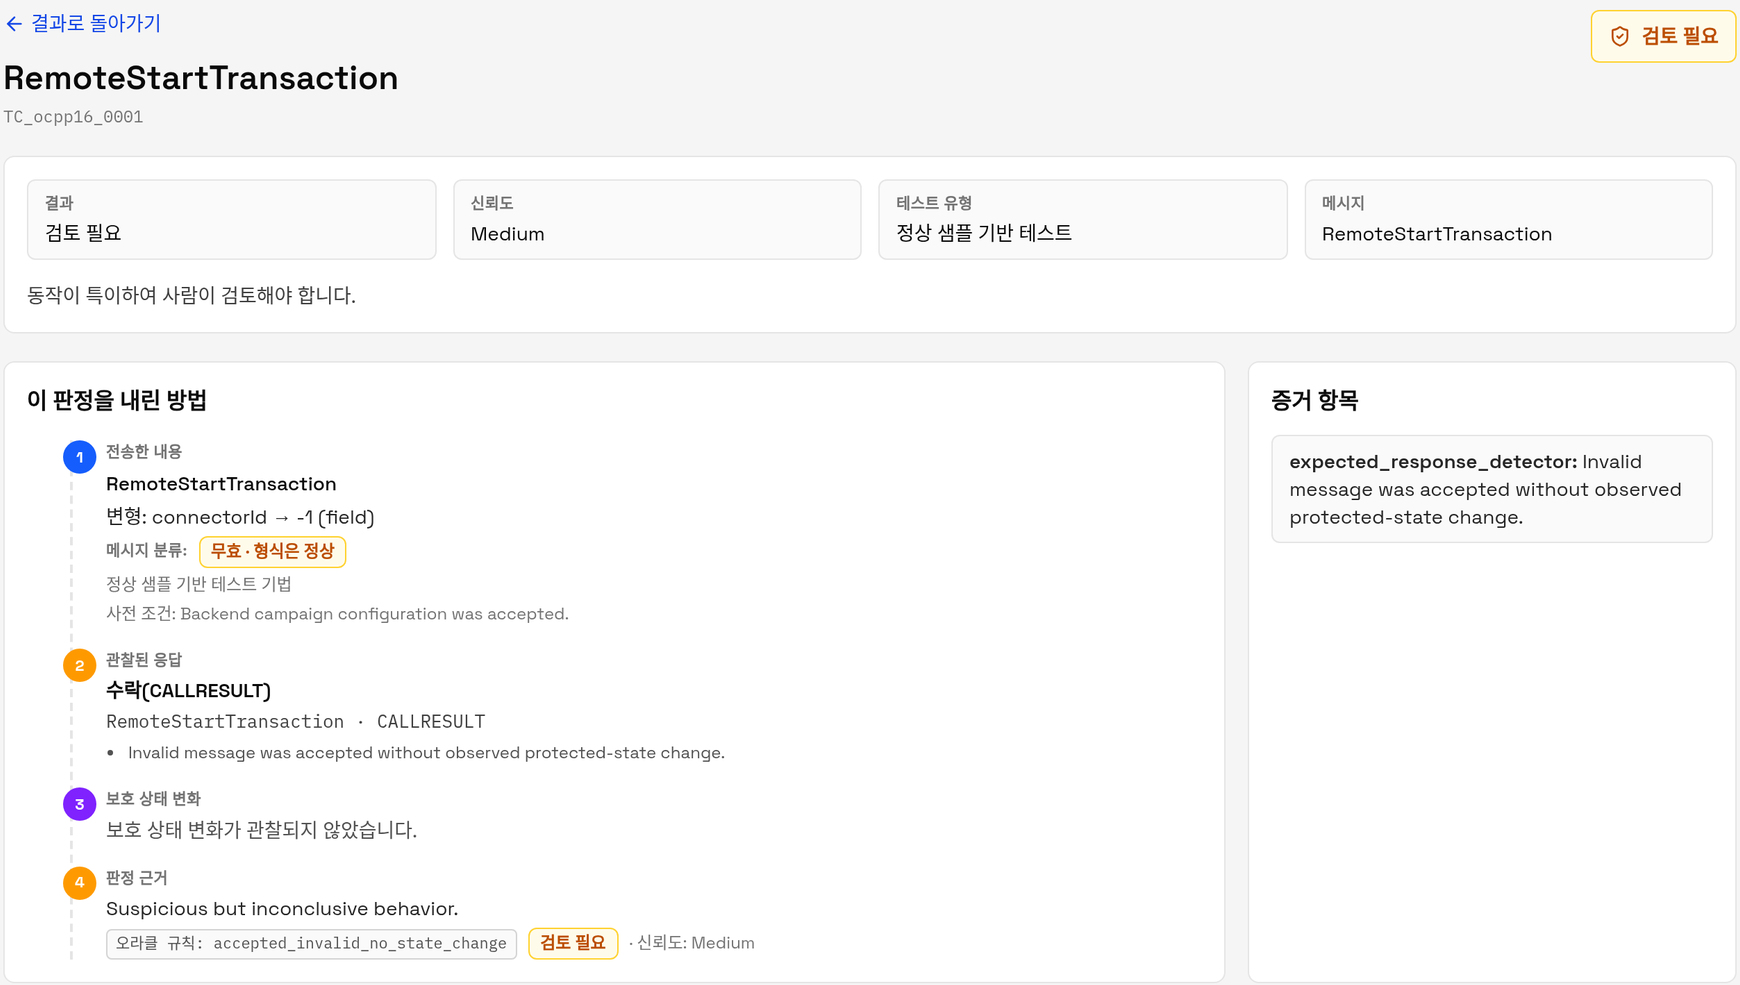
\includegraphics[width=\textwidth]{screenshots/ui04_detail_c.png}
    \caption{웹 화면: 개별 결과의 판정 근거}
    \label{fig:ui-detail}
\end{figure}

\subsection{판정 기준표}

표~\ref{tab:matrix}는 입력의 의도와 관측 결과의 조합별 판정이다.
핵심 원칙은 \textbf{잘못된 입력이 수락된 것만으로는 결함으로 보지 않고, 보호 상태가 실제로 바뀐 근거가 있을 때만 잠재 이슈로 올린다}는 것이다.
이 원칙은 블랙박스 퍼징에서 흔한 오탐(false positive)을 줄이기 위한 것이다.

\begin{table}[H]
\centering
\small
\caption{입력 의도 $\times$ 응답 $\times$ 상태 변화 판정표}
\label{tab:matrix}
\renewcommand{\arraystretch}{1.3}
\begin{tabularx}{\textwidth}{>{\raggedright\arraybackslash}p{3.6cm} Y Y Y}
\toprule
\textbf{입력의 의도} & \textbf{수락,\newline 상태 변화 없음} & \textbf{수락,\newline 보호 상태 변화} & \textbf{프로토콜 오류로 거부} \\
\midrule
정상 메시지 & 통과 & 통과\newline{\scriptsize (세션 규칙 위반 시 잠재 이슈)} & 실패 \\
형식은 맞지만 부적합 & 검토 필요 & 잠재 이슈 & 안전하게 거부됨\newline{\scriptsize (상태가 바뀌었으면 잠재 이슈)} \\
형식이 깨진 메시지 & 검토 필요 & 잠재 이슈 & 안전하게 거부됨 \\
정책에 따라 다름\newline(정책 정보 없음) & 검토 필요 & 검토 필요\newline{\scriptsize (트랜잭션이 생성되면 잠재 이슈)} & 안전하게 거부됨 \\
\bottomrule
\end{tabularx}
\end{table}

무응답과 연결 끊김은 크래시나 멈춤의 징후일 수 있지만 네트워크 지연일 수도 있으므로 검토 필요로 분류하고, 상태 확인과 복구가 반복 실패한 경우는 응답 불능으로 별도 기록한다.

\subsection{상태 불변식}\label{subsec:invariants}

상태 불변식은 입력의 종류와 무관하게 충전 세션이 항상 지켜야 하는 규칙이다.

\begin{itemize}
    \item 거부된 입력은 보호 상태를 바꾸지 않아야 한다.
    \item 잘못된 커넥터 번호로 트랜잭션이 만들어져서는 안 된다.
    \item 인증 없이 트랜잭션이 시작되어서는 안 된다.
    \item 진행 중인 트랜잭션이 있는데 두 번째 트랜잭션이 생겨서는 안 되고, 진행 중인 트랜잭션 없이 종료가 성공해서도 안 된다.
    \item 트랜잭션 번호는 대상이 발급한 값과 일치하고 세션 동안 유지되어야 한다.
\end{itemize}

이 중 인증 없는 트랜잭션 시작, 트랜잭션 수명주기 위반, 트랜잭션 번호 불일치는 \textbf{입력의 의도와 무관한 위반}으로, 정상 메시지에서 발생하더라도 잠재 이슈로 보고한다.

\subsection{대상 정책 프로파일}

일부 변형은 대상의 운영 정책에 따라 정답이 달라진다. 어떤 인증 태그가 등록되어 있는지, 몇 번 커넥터가 있는지, 어떤 기능을 지원하는지가 그 예이다.
대상 정책 프로파일은 이러한 정보를 시험 전에 기술해 두는 것으로, 판정 단계에서 입력의 의도를 대상에 맞게 재분류하는 데 쓰인다.
예를 들어 프로파일에 등록된 태그는 정상 메시지로, 지원하지 않는 기능의 명령은 거부되어야 하는 입력으로 다시 분류된다.
프로파일이 없을 때 정책에 따라 다른 입력이 수락되면 결론을 내리지 않고 낮은 신뢰도의 검토 필요로 남긴다.

\subsection{ISO 15118 판정}

ISO 15118에도 같은 판정 모델을 적용한다.
전송 계층에서는 프레임 헤더와 인코딩의 유효성을 확인하고, 세션 계층에서는 표준 협상 순서(세션 설정 $\rightarrow$ 서비스 협상 $\rightarrow$ 결제 방식 선택 $\rightarrow$ 인증 $\rightarrow$ 충전 조건 협상 $\rightarrow$ 전력 공급 $\rightarrow$ 종료)를 기준으로 다음을 검사한다.

\begin{itemize}
    \item 요청에 맞지 않는 종류의 응답
    \item 수립된 세션과 다른 세션 식별자의 사용 또는 세션 식별자의 변경
    \item 인증 전에 충전 조건 협상이나 전력 공급이 성공하는 경우
    \item 협상 순서를 건너뛴 요청이 성공하는 경우
\end{itemize}
